\begin{frame}{Aerodynamic Duty}

    The aerodynamic duty is a way of expressing the \textbf{macroscopic flow deflection properties} that the blade has to generate.

    \begin{columns}
        \column{0.5\textwidth}
        \vspace{0.5cm}
        \begin{block}{System constraints}
            \begin{itemize}
                \setlength\itemsep{0.3cm}
                \item $\alpha_1$: inlet flow angle
                \item $\alpha_2$: outlet flow angle
                \item $M_2$: outlet flow Mach number after mixout
                \item $Re$: Reynolds number of the flow
            \end{itemize}
        \end{block}
        \column{0.5\textwidth}
            \vspace{-0.5cm}
            % \begin{figure}
                % 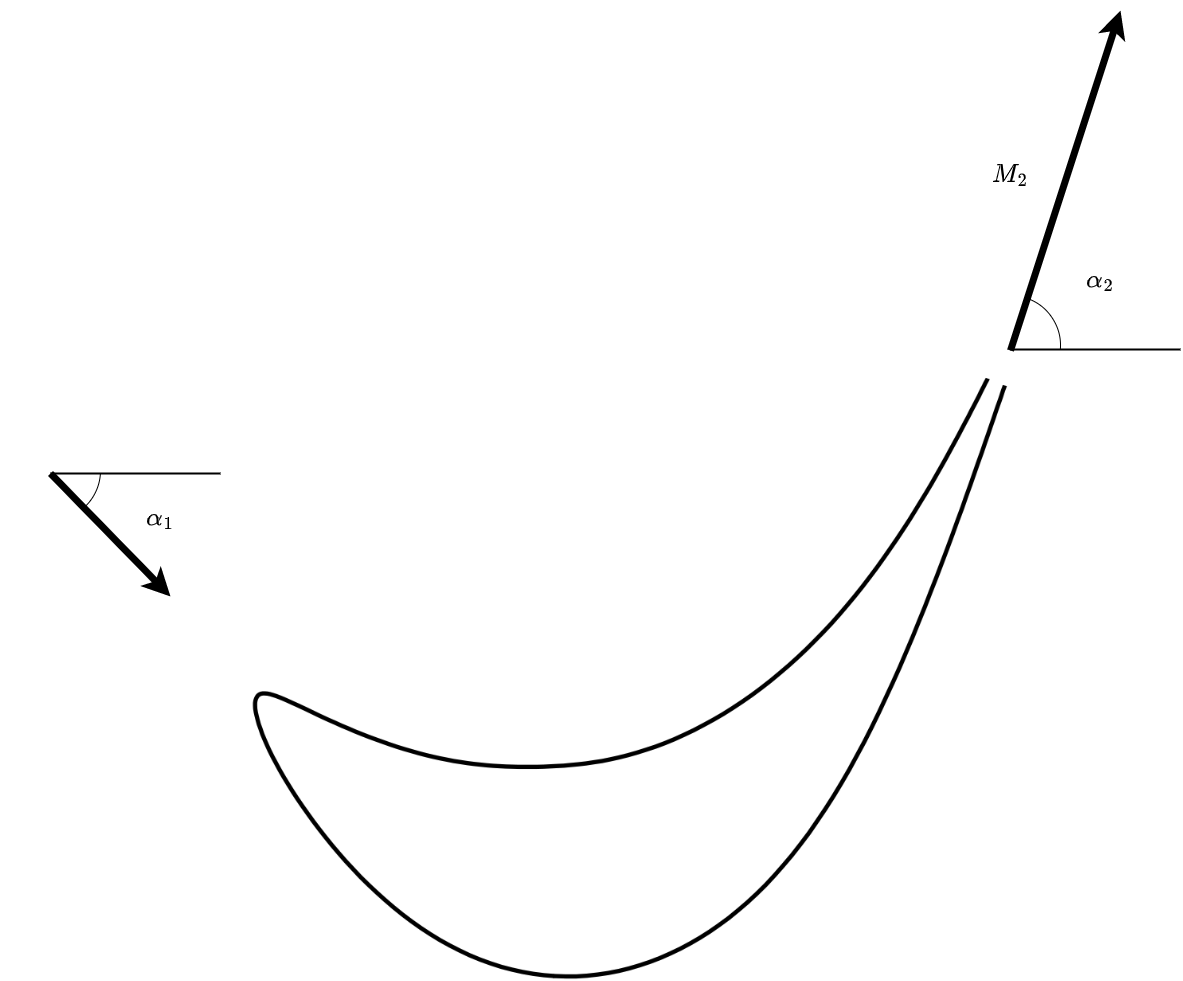
\includegraphics[width=\textwidth]{images/aeroDuty.png}
            % \end{figure}
            \begin{figure}[!h]

    \begin{center} 
    
        \begin{tikzpicture}
            \begin{axis}[
                width=0.5\textwidth, % Increased width
                axis equal,          % Set equal aspect ratio
                axis lines=none,     % Remove axis lines and labels
                xmin=-0.3, xmax=1.3, % Increased x limits
                ymin=-0.1, ymax=1.6,   % Increased y limits
            ]

            \addplot[black, line width=2pt] table[x index=0, y index=1, col sep=comma] {./pyFigure/csv/coords.csv};
            \addplot[black, line width=2pt] table[x index=2, y index=3, col sep=comma] {./pyFigure/csv/coords.csv};
            
            % Adding the second arrow with text
            \draw[-latex, line width=2.5pt] (axis cs:-0.25,0.55) -- node[below left] {$Re$} (axis cs:-0.05,0.35);
            \draw[-latex, line width=2.5pt] (axis cs:1.02,1) -- node[above left] {$M_2$} (axis cs:1.22,1.6);
            \draw[-, line width=1.0pt] (axis cs:-0.25,0.55) -- node[below] {$\alpha_1$} (axis cs:0.15, 0.55);
            \draw[-, line width=1.0pt] (axis cs:1.02,1) -- node[above left] {$\alpha_2$} (axis cs:1.45, 1);
            
            \end{axis}
        \end{tikzpicture}
    
    \end{center}

    \caption{Aerodynamic duty parameters.}
    \label{fig:aeroDuty}

\end{figure}
    \end{columns}
    
    % \begin{alertblock}{DOF properties}
        % \begin{itemize}
            % \item This is the value after the flow has mixed out at the end of the blade
            % \item The simulations are made using high Reynolds numbers, this in order to prevent flow separation (due to the switch to turbulente boundary layer)
        % \end{itemize}    
    % \end{alertblock}
\end{frame}